\documentclass[12pt]{beamer}
\geometry{paper=a6paper,landscape}

\usetheme{default}% I recommend
% \or\usetheme{Singapore}
% \or\usetheme{Boadilla}
% \or\usetheme{Pittsburgh}
% \or\usetheme{Madrid}
% \or\usetheme{Warsaw} % common choice, but often poor
% \fi

\usepackage{graphicx,pgfplots,parskip}
\usepackage{listings}
\usepackage{semantic}
\usepackage[utf8]{inputenc}
\usepackage[T1]{fontenc}
\usepackage{microtype}
\usepackage{amsmath}
\usepackage{amssymb}
\usepackage{ifthen}
\newcommand\hmmax{0} % default 3
% \newcommand\bmmax{0} % default 4
% \usepackage{bm}
\usepackage{stmaryrd}
\usepackage{proof}
\usepackage{graphicx}
\usepackage[export]{adjustbox}
\usepackage{listings}
\usepackage{tikz}
\usepackage{semantic}
\usepackage{setspace}
\usepackage{wrapfig}
\usepackage{color}
\usepackage{caption}
\usepackage{subcaption}
\usepackage{esvect}
\usepackage{tikz}
\usepackage{booktabs} %% http://ctan.org/pkg/booktabs
\usepackage{wasysym}
\usepackage{array,multirow}
\usepackage{balance}
\usepackage[backend=bibtex, style=authoryear-comp]{biblatex}

%%%%%%%%%%%%%%%%%%%%% MACROS %%%%%%%%%%%%%%%%%%%%%%%%%%%


\definecolor{lightgray}{gray}{0.9}
%\newcommand{\highlight}[1]{\colorbox{lightgray}{$\displaystyle #1$}}
\newcommand{\hi}[1]{\colorbox{lightgray}{$\displaystyle #1$}}

\newcommand{\tagsc}[1]{\tag{\textsc{#1}}}
\newcommand{\newname}[2]{\newcommand{#1}{\ensuremath{#2}}}

\newcommand{\overbar}[1]{\mkern 1.5mu\overline{\mkern-1.5mu#1\mkern-1.5mu}\mkern 1.5mu}

\newcommand{\size}{size}
\newcommand{\cast}{\Rightarrow}
\newcommand{\CoercionTyping}{\Longrightarrow}
\newcommand{\castE}[4][]{\ensuremathc{#2 : #3 \Rightarrow^{#1} #4}}

\newcommand{\key}[1]{\texttt{#1}}

% Types
\newcommand{\UnitT}{\ensuremath{\mathsf{()}}}
\newcommand{\IntT}{\ensuremath{\mathsf{Int}}}
\newcommand{\BoolT}{\ensuremath{\mathsf{Bool}}}
\newcommand{\DynT}{\ensuremath{\mathsf{\star}}}
\newcommand{\RefT}[1]{\ensuremath{\mathsf{Ref}\ #1}}
\newcommand{\RefPT}[1]{\ensuremath{\mathsf{Ref}\ #1}}
%\newcommand{\RefMT}[1]{\ensuremath{\mathsf{Ref}_m #1}}
\newcommand{\FunT}[2]{\ensuremath{#1 \to #2}}
\newcommand{\CFunT}[3]{\ensuremath{(\overbar{#1},#2) \cast #3}}
\newcommand{\TupleT}[2]{\ensuremath{#1 \times #2}}
\newcommand{\Unit}{\ensuremath{\text{Unit}}}
\newcommand{\CClosT}[2]{\ensuremath{#1 \to #2}}
\newcommand{\CoT}[2]{\ensuremath{#1 \Longrightarrow #2}}

\newcommand{\IntC}{\ensuremath{\mathtt{Int}}}
\newcommand{\BoolC}{\ensuremath{\mathtt{Bool}}}
\newcommand{\DynC}{\ensuremath{\mathtt{Dyn}}}
\newcommand{\RefC}[1]{\ensuremath{\mathtt{Ref}\ #1}}

% Relations

\newcommand{\TypePreciseness}{\sqsubseteq}
\newcommand{\ExprTypePreciseness}{\sqsubseteq}
\newcommand{\StoreTypePreciseness}{\sqsubseteq_p}
\newcommand{\StoreTypeExtension}{\sqsubseteq_e}
\newcommand{\StoreTypeEvolution}{\sqsubseteq_{p/e}}
\newcommand{\static}{\Rbag}
\newcommand{\ShallowConsist}{\small\smile}

% Coercions
\newcommand{\idC}{\ensuremath{\mathtt{\iota}}}
\newcommand{\InjectCoercion}[1]{\ensuremath{#1!}}
\newcommand{\seqInjC}[2]{\ensuremath{\seqC{#1}{\InjectCoercion{#2}}}}
\newcommand{\ProjectCoercion}[1]{\ensuremath{#1?}}
\newcommand{\seqPrjC}[2]{\ensuremath{\seqC{\ProjectCoercion{#1}}{#2}}}
\newcommand{\FunctionCoercion}[2]{\ensuremath{#1 \to #2}}
\newcommand{\RefCoercion}[1]{\ensuremath{\mathsf{Ref}\ #1}}
\newcommand{\seqC}[2]{\ensuremath{#1 \, ; \, #2}}
\newcommand{\FailCoercion}[2]{\ensuremath{\bot^{#1#2}}}
\newcommand{\FailCoercionSE}{\ensuremath{\bot}}
\newcommand{\TupleCoercion}[2]{\ensuremath{#1 \times #2}}

\newcommand{\coercion}[1]{\ensuremath{\langle #1 \rangle}}
\newcommand{\coerce}[2]{\ensuremath{#1 \coercion{#2}}}
\newcommand{\coerced}[2]{\ensuremath{\coerce{#1}{#2}}}
\newcommand{\app}[2]{\ensuremath{#1 \, #2}}
\newcommand{\lam}[2]{\ensuremath{\lambda #1 . #2}}
\newcommand{\blame}[1]{\ensuremath{\mathtt{blame}\, #1}}
\newcommand{\mkRef}[1]{\ensuremath{\mathtt{ref}\ #1}}
\newcommand{\allocT}[2]{\ensuremath{\mathtt{ref}\ #1 @ #2}}
\newcommand{\alloc}[1]{\allocT{#1}{\AllTa}}
\newcommand{\deref}[1]{\ensuremath{\mathtt{!} #1}}
\newcommand{\derefT}[1]{\ensuremath{\mathtt{!} #1 @ \AllTa}}
\newcommand{\DerefT}[2]{\ensuremath{\mathtt{!} #1 @ #2}}
\newcommand{\setref}[2]{\ensuremath{#1\ {:=}\ #2}}
\newcommand{\setrefT}[2]{\ensuremath{#1\ {:=}\ #2 @ \AllTa}}
\newcommand{\SetrefT}[3]{\ensuremath{#1\ {:=}\ #2 @ #3}}
\newcommand{\error}{\ensuremath{\mathtt{error}}}
\newcommand{\Error}{\ensuremath{\mathtt{Err}}}
\newcommand{\dom}[1]{\ensuremath{\text{dom}(#1)}}
\newcommand{\tuple}[2]{\ensuremath{(#1,#2)}}
\newcommand{\fst}[1]{\ensuremath{(\mathtt{fst}\, #1)}}
\newcommand{\snd}[1]{\ensuremath{(\mathtt{snd}\, #1)}}

\newcommand{\glbt}{\sqcap}

\newcommand{\var}[1][x]{\ensuremath{#1}}
\newcommand{\expr}[1][e]{\ensuremath{#1}}
\newcommand{\const}{\ensuremath{k}}

\newcommand{\uncoerced}{\ensuremath{u}}
\newcommand{\val}{\ensuremath{v}}
\newcommand{\CastedValueA}{\ensuremath{cv}}
\newcommand{\CastedValueB}{\ensuremath{cv'}}
\newcommand{\CastedValueC}{\ensuremath{cv''}}
\newcommand{\StrongCastedVal}{\ensuremath{cv^{+}}}

\newcommand{\hole}{\ensuremath{\square}}
\newcommand{\context}[2]{\ensuremath{ #1 [ #2 ] }}

\newcommand{\InertCoercion}[1]{\ensuremath{#1\uparrow}}
\newcommand{\InertCoercionA}{\InertCoercion{\seCa}}
\newcommand{\InertCoercionB}{\InertCoercion{\seCb}}
\newcommand{\InertFinalCoercion}{\ensuremath{\seFinalC\uparrow}}
\newcommand{\InertMiddleCoercion}{\ensuremath{\seInterC\uparrow}}
\newcommand{\ActiveCoercion}[1]{\ensuremath{#1\downarrow}}
\newcommand{\ActiveCoercionA}{\ActiveCoercion{\seCa}}
\newcommand{\ActiveCoercionB}{\ActiveCoercion{\seCb}}
\newcommand{\ActiveFinalCoercion}{\ensuremath{\seFinalC\downarrow}}
\newcommand{\ActiveMiddleCoercion}{\ensuremath{\seInterC\downarrow}}

\newcommand{\CastCong}{\varphi}
\newcommand{\AllowCastCong}{\top}
\newcommand{\DisallowCastCong}{\bot}
\newcommand{\PureSymbol}{\obslash}
\newcommand{\ImpureSymbol}{\ocircle}
\newcommand{\PureCastReduce}{\longrightarrow_{c}^{\PureSymbol}}
\newcommand{\PureCastCastedValueReduce}{\longrightarrow_{cv}^{\PureSymbol}}
\newcommand{\MonoCastReduce}{\longrightarrow_{c}^{\ImpureSymbol}}
\newcommand{\CastReduce}{\longrightarrow_{c}}
\newcommand{\CastedValueReduce}{\longrightarrow_{cv}}
\newcommand{\PureReduce}{\longrightarrow_{e}^{\PureSymbol}}
\newcommand{\MonoReduce}{\longrightarrow_{e}^{\ImpureSymbol}}
\newcommand{\ProgReduce}{\longrightarrow_{e}}
\newcommand{\Lang}{\ensuremath{\textsc{GTLC}^{+}}}

% Meta Variables
\newname{\BaseT}{B}
\newname{\InjTa}{I}
\newname{\InjTb}{J}
\newname{\AllTa}{T}
\newname{\AllTb}{S}
\newname{\topC}{c}
\newname{\noFailC}{r}
\newname{\blameLabel}{p}
\newname{\addr}{a}
\newname{\seCa}{c}
\newname{\seCb}{d}
\newname{\ca}{c}
\newname{\cb}{d}
\newname{\seFinalC}{i}
\newname{\seInterC}{g}
\newname{\seIdFreeC}{f}
\newname{\CoercionT}{\mathcal{C}}
\newname{\expra}{M}
\newname{\exprb}{N}
\newname{\ctag}{w}
\newname{\uctag}{uc}
\newname{\cctag}{cc}

% Functions
\newcommand{\ComposeCoercion}{\fatsemi}
\newcommand{\ComposeMiddleCoercion}{\ensuremath{\fatsemi_{\text{\tiny g}}}}
\newcommand{\ComposeFinalCoercion}{\ensuremath{\fatsemi_i}}
\newcommand{\mkC}[2]{\ensuremath{ #1 \Rightarrow #2 }}

\newcommand{\jdgt}[2]{\ensuremath{\Gamma\vdash #1:#2}}
\newcommand{\ctit}[3]{\ensuremath{\Gamma\vdash #1 \hookrightarrow #2:#3}}
\newcommand{\mkCrcn}[2]{\ensuremath{\langle #1 \Longrightarrow #2
    \rangle}}

% Heaps
\newcommand{\store}{\ensuremath{\mu}}
\newcommand{\evstore}{\ensuremath{\nu}}
\newcommand{\storecell}[1]{\ensuremath{\addr \mapsto #1}}
\newcommand{\mstorecell}[2]{\ensuremath{\addr \mapsto #1 : #2}}
\newcommand{\StoreCell}[3]{\ensuremath{#1 \mapsto #2 : #3}}
\newcommand{\StoreValRead}{\ensuremath{\store(\addr)_{\text{val}}}}
\newcommand{\StoreRTTIRead}{\ensuremath{\store(\addr)_{\text{rtti}}}}
\newcommand{\EvStoreValRead}{\ensuremath{\evstore(\addr)_{\text{val}}}}
\newcommand{\EvStoreRTTIRead}{\ensuremath{\evstore(\addr)_{\text{rtti}}}}

\newcommand{\EvolvingStoreRTTIRead}[2]{\ensuremath{#1(#2)_{\text{rtti}}}}


\DeclareCiteCommand{\citeseries}
  {\usebibmacro{prenote}}
  {\usebibmacro{citeindex}%
    \printfield{series}}
  {\multicitedelim}
  {\usebibmacro{postnote}}

\addbibresource{all.bib}

\newcommand{\customcite}[1]{\citeauthor{#1}, \citetitle{#1},
  \citeseries{#1} \citeyear{#1}}

\newcommand{\customcitewithoutseries}[1]{\citeauthor{#1},
  \citetitle{#1}, \citeyear{#1}}

\lstdefinestyle{basic}{
%showstringspaces=false,
language=Python,
columns=fullflexible,
%basicstyle=\sffamily\small,%
basicstyle=\ttfamily,%
%columns=fixed,
%basewidth=0.49em,
%lineskip=0pt,
%escapechar=@,xleftmargin=1pc,%
keywordstyle=\ttfamily,
mathescape=true,%
moredelim=**[is][\color{blue}]{@}{@},
moredelim=[is][\color{red}]{|}{|},
moredelim=[is][\color{blue}]{~}{~},
%commentstyle=\rmfamily,%
%morekeywords={return,fix,var,proc,fun,func},%
%deletekeywords={int,bool}
}
\lstset{style=basic}

\newcommand{\lstsetgrift}{
  \lstset{%
    language=Lisp,
    numbers=left,
    stepnumber=1,
    basicstyle=\ttfamily\small,
    keywordstyle=\ttfamily\bfseries\small,
    columns=flexible,
    aboveskip=\smallskipamount,
    belowskip=\smallskipamount,
    xleftmargin=2pt,
    escapeinside={/+}{+/},
    mathescape=true,
    morekeywords=[1]{define,lambda,if,begin,letrec,let,let*,values,:,repeat,then,else,return,and,time,box,ref,unbox,box,ann},
    literate=
    {+}{{\textsf{+}}}1
    {-}{{\textsf{-}}}1
    {=>}{{$\rightarrow\;$}}2
    {lambda}{{$\boldsymbol{\lambda}$}}1
  }
}%%


\title{Toward Efficient Gradual Typing}
\author{Deyaaeldeen Almahallawi\\
  Bloomberg, Indiana University}

\date{July 2019}

\begin{document}

\begin{frame}
\maketitle
\end{frame}

\frame{
\frametitle{Toward Efficient Gradual typing for Structural Types via
  Coercions, PLDI 2019}
\begin{center}
  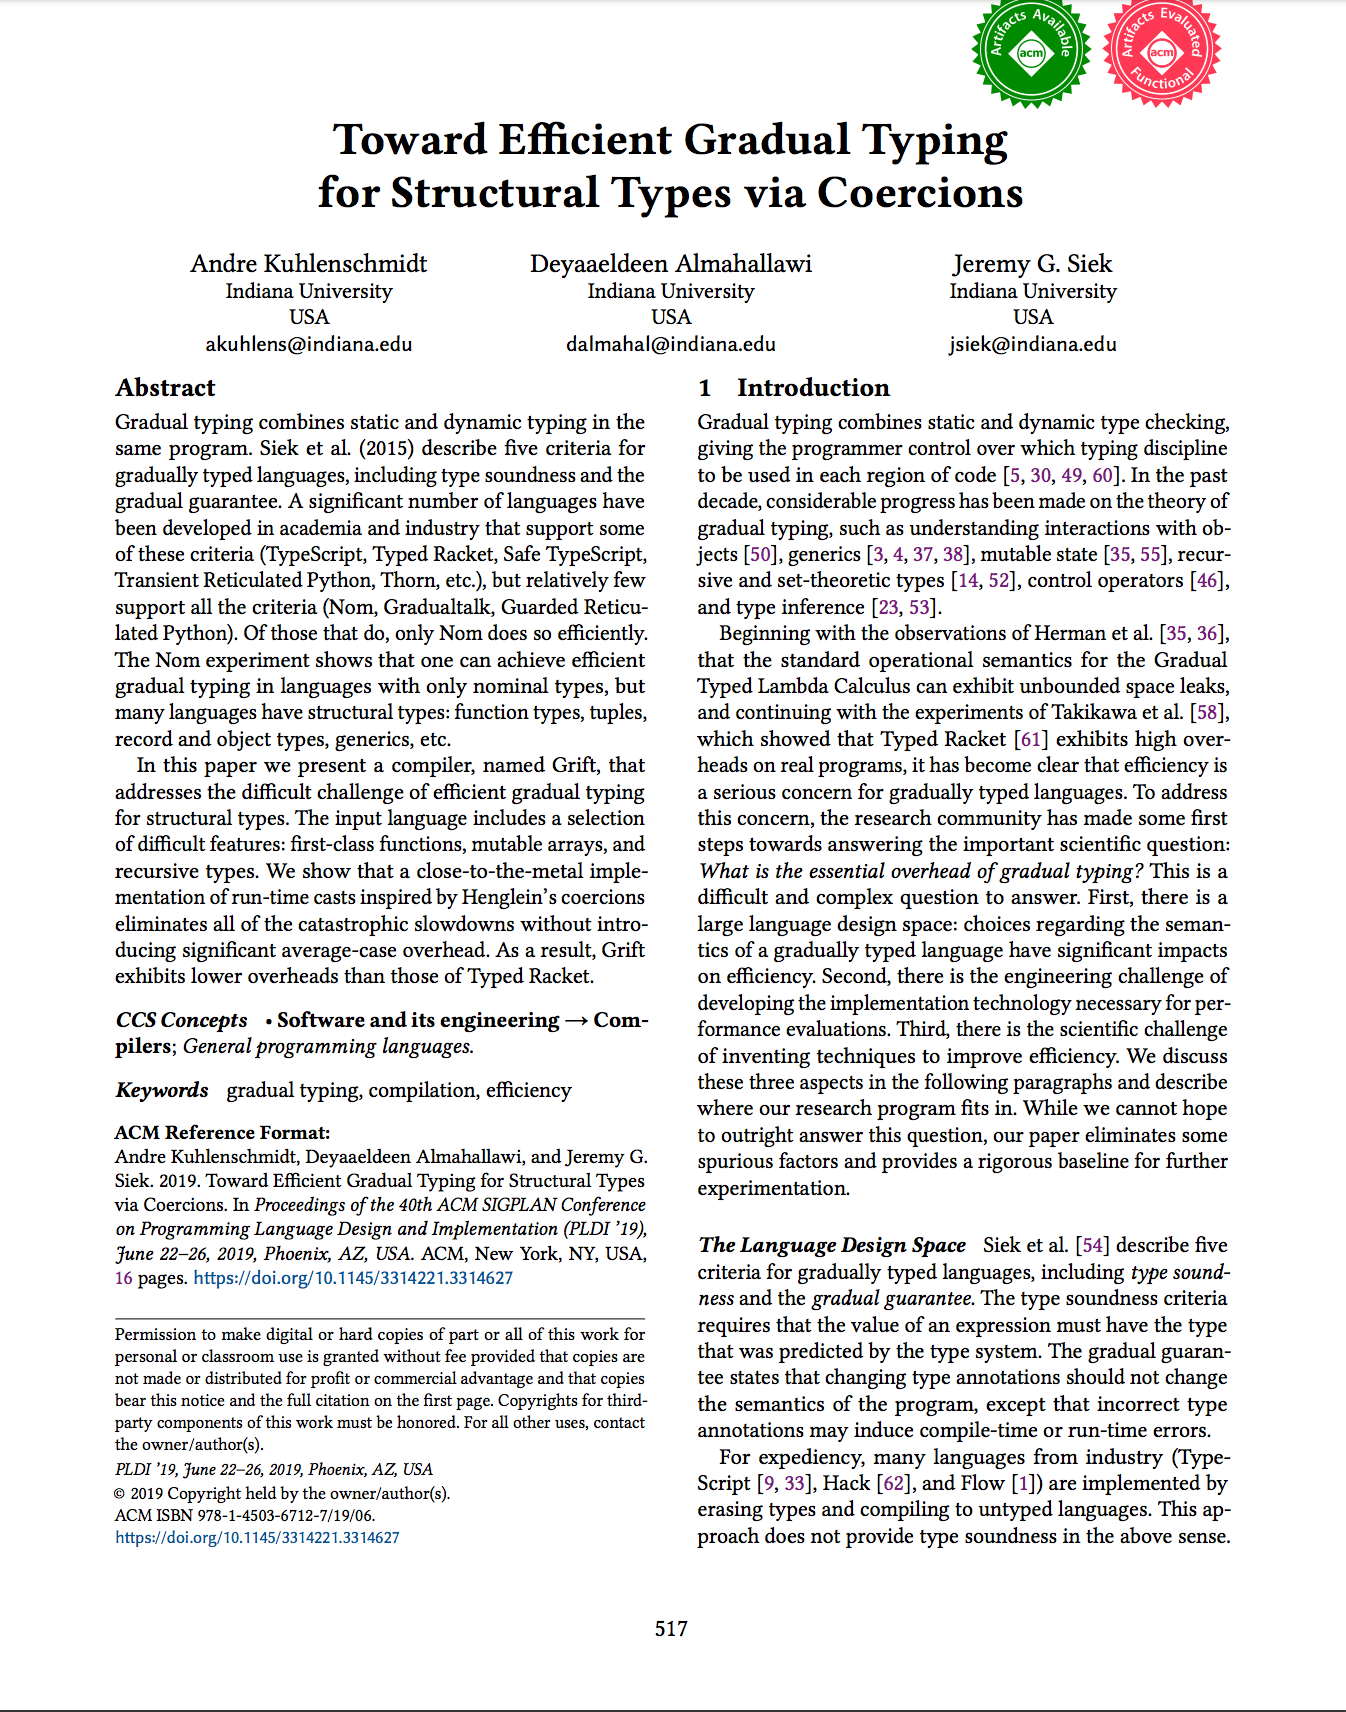
\includegraphics[scale=0.2]{paper.png}
\end{center}
}

\frame{
\frametitle{Gradual typing}
\begin{center}
  
\includegraphics{yinyang.png}
\end{center}
}

\begin{frame}{Outline}
\tableofcontents
\end{frame}

\section{Introduction}

\begin{frame}{Industry adoption}

  \begin{itemize}
  \item TypeScript, C\# (Microsoft)
  \item Flow, Hack, Pyre (Facebook)
  \item Dart (Google)
  \item Sorbet (Stripe)
  \end{itemize}
\end{frame}

\begin{frame}{What is NOT gradual typing}

  \begin{itemize}
  \item type inference
  \item type hints
  \item optional typing (type erasure)
  \end{itemize}
\end{frame}

\begin{frame}{History of Gradual Typing}
  \begin{itemize}
  \item \customcite{Siek:2006bh}
  \item \customcite{Tobin-Hochstadt:2006fk}
  \end{itemize}
\end{frame}

\begin{frame}[fragile]
\frametitle{Gradual typing preserves soundness}
\note{Gradual typing has two compelling features: soundness and interoperability}
\begin{center}
\note{Regarding soundness, programmers, compilers, and IDEs would like
  to trust their type annotations}
\begin{lstlisting}
(define (f [x : Int]) (+ x 1))
\end{lstlisting}
\note{this expression should be accepted}
\pause
\begin{lstlisting}
(f 1)
\end{lstlisting}
\note{this expression should be rejected}
\pause
\begin{lstlisting}
(f 0.5)
\end{lstlisting}
\pause
\begin{lstlisting}
(define (g y) (f y))
\end{lstlisting}
\pause
\begin{lstlisting}
(g 1)
(g 0.5)
\end{lstlisting}
\end{center}

\end{frame}

\begin{frame}{Type system}

\fbox{$\Gamma \vdash_s e : T$}
\begin{gather*}
  \inference{\Gamma\vdash_s\expra:\FunT{\AllTa_1}{\AllTa_2} &
    \Gamma\vdash_s\exprb:\AllTa_1}{\Gamma\vdash_s\app{\expra}{\exprb}:\AllTa_2}
\end{gather*}
\pause
Consistency \hfill \fbox{$\AllTa \sim \AllTa$}
\begin{gather*}
\DynT \sim \AllTa
\qquad
\AllTa \sim \DynT
\qquad
\BaseT \sim \BaseT
\qquad
\inference
  {\AllTa_1 \sim \AllTa_3 & \AllTa_2 \sim \AllTa_4}
  {\AllTa_1 \to \AllTa_2 \sim \AllTa_3 \to \AllTa_4}
\end{gather*}

\fbox{$\Gamma \vdash_g e : T$}
\begin{gather*}
  \inference{\Gamma\vdash_g\expra:\AllTa &
    \Gamma\vdash_g\exprb:\AllTa' & arg(\AllTa) \sim
    \AllTa'}{\Gamma\vdash_g\app{\expra}{\exprb}:return(\AllTa)}
  \\[2ex]
  arg(\FunT{\AllTa_1}{\AllTa_2}) = \AllTa_1 \qquad   arg(\DynT) = \DynT
  \\
  return(\FunT{\AllTa_1}{\AllTa_2}) = \AllTa_2 \qquad   return(\DynT) = \DynT
\end{gather*}

\end{frame}

\frame{
\frametitle{Cast insertion}

\fbox{$\Gamma \vdash e \leadsto e' : T$}
\begin{gather*}
\inference
    {\Gamma \vdash e_1 \leadsto e'_1 : \FunT{T_1}{T_2} &
      \Gamma \vdash e_2 \leadsto e'_2 : T_1' \\
      T_1 \sim T_1'}
    {\Gamma \vdash \app{e_1}{e_2} \leadsto (\app{e'_1}{(\coerced{e'_2}{T_1' \cast T_1})}) : T_2}
\\[5ex]
\inference{\Gamma \vdash e_1 \leadsto e'_1 : \DynT & 
  \Gamma \vdash e_2 \leadsto e'_2 : T}
          {\Gamma \vdash e_1 \app e_2 \leadsto 
            \app{(\coerced{e_1}{\DynT \cast
                \FunT{\DynT}{\DynT}})}{\coerced{e_2}{\AllTa \cast \DynT}}}
\end{gather*}

}

\frame{
\frametitle{Operational semantics of casts} % UD

\note{higher order casts are problematic because they can accumulate}

\[
\begin{array}{llcl}
\text{Values} & v &::= &\dots \mid \lam{\var : \AllTa}{e} \mid
                         \coerced{\val}{\AllTa_1 \cast \AllTa_2}
\end{array}
\]

\begin{align*}
  (\coerced{\val}{\FunT{\AllTa_1}{\AllTa_2} \cast \FunT{\AllTa_1'}{\AllTa_2'}})\app v' & \longrightarrow
                                                                                         \coerced{(\app{\val}{(\coerced{\val'}{T'_1 \cast  T_1})})}{T_2 \cast T'_2} \\
\end{align*}
}

\begin{frame}
  \begin{theorem}[Gradual Guarantee]
Suppose $e \TypePreciseness e'$ and $\vdash e : T$.
\begin{enumerate}
\item $\vdash e':T'$ and $T \TypePreciseness T'$.
\item If $e\Downarrow v$, then $e'\Downarrow v'$ and $v \TypePreciseness v'$.\\
      If $e\Uparrow$ then  $e'\Uparrow$.
\item If $e'\Downarrow v'$, then $e\Downarrow v$ 
      where $v \TypePreciseness v'$, or $e \Downarrow \key{blame}_T\ l$.\\
      If $e'\Uparrow$, then $e\Uparrow$ or $e \Downarrow \key{blame}_T\ l$.
 \end{enumerate}
\end{theorem}
\end{frame}

\frame{
  \tiny
  \begin{tabular}{ccccc|cc}
    \multicolumn{2}{c}{}
    & \multicolumn{2}{c}{Gradual Guarantee wrt.}
    & \multicolumn{1}{c}{} \\
    Language
%    & Implementation
    & Sound
    & Structural Types & Nominal Types
    & Granularity
    & Approach
    & Space-Efficient \\
    \hline 
    Gradualtalk
    & \CIRCLE & \CIRCLE & \CIRCLE & Fine & Retrofit & \Circle \\
    Guarded Reticulated Python
    & \CIRCLE & \CIRCLE & \CIRCLE & Fine & Retrofit & \Circle\\
    Nom
%    & Nom Compiler
    & \CIRCLE & -- & \CIRCLE & Fine & From-Scratch & \CIRCLE \\
    GTLC+
%    & Grift
    & \CIRCLE & \CIRCLE & -- & Fine & From-Scratch & \CIRCLE \\
    \hline
    TypeScript
%    & TypeScript Compiler
    & \Circle
    & \CIRCLE  % TypeScript? If so, then removing types
    & \CIRCLE  % can lead static failures.
    & Fine & Retrofit
    & \CIRCLE
    \\
    Safe TypeScript
%    & Higgs VM \& JIT
    & \CIRCLE
    & \Circle 
    & \Circle % ¬(e1 : {m(C) : Bool}, e2 : Any ⊢ e1.m(e2)) since ¬(Any <: C)
    & Fine & Retrofit
    & \CIRCLE
    % nominal types, but the text mentions them.
    \\
    Typed Racket
%    & Racket VM
    & \CIRCLE & \LEFTcircle & \LEFTcircle % Structs are nominal
    & Coarse & Retrofit
    & \CIRCLE \\ 
    %% Typed-Racket & Pycket
    %% & \CIRCLE & \CIRCLE & \CIRCLE % Structs are nominal
    %% & \Circle \\ 
    %% \hline
    Transient Reticulated Python
    & \LEFTcircle & \CIRCLE & \CIRCLE
    & Fine & Retrofit
    & \CIRCLE
  \end{tabular}

  }


\section{Performance Problems}

\begin{frame}{Outline}
\tableofcontents[currentsection]
\end{frame}

\frame{
\frametitle{Casts can cause catastrophic slowdowns}

\note{ for most of their benchmarks that the worst performing
  configurations spend > 80% of their runtime
  executing casts. The majority of these casts are casts on values of
  higher-order types}

\note{claim that sound gradual typing is dead in the context of the
  current implementation technologies.}

\begin{center}
%
\includegraphics[width=3.5in]{sound-dead}\\
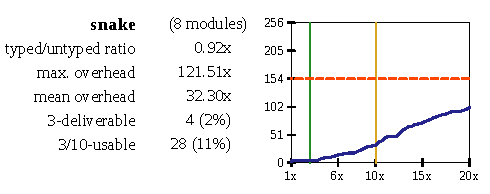
\includegraphics[width=3.5in]{snake} \\
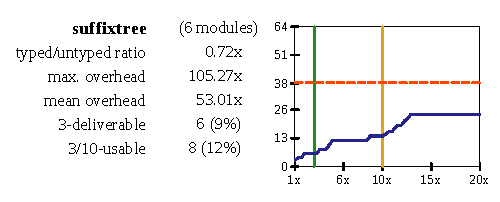
\includegraphics[width=3.5in]{suffixtree}
\end{center}

\footnote{\textit{Is sound gradual typing dead?}
  Takikawa et al. POPL 2016}

}

\begin{frame}[fragile]
\frametitle{Casts can cause catastrophic slowdowns}

\begin{center}
\begin{lstlisting}
(define sort!
  : ((Vectorof Dyn) Int Int -> ())
  (lambda ([v : (Vectorof Int)]
       [lo : Int][hi : Int])
    (when (< lo hi)
      (let ([pivot : Int (partition! v lo hi)])
        (sort! v lo (- pivot 1))
        (sort! v (+ pivot 1) hi)))))
\end{lstlisting}
\end{center}

\end{frame}

%===============================================================================
\frame{
\frametitle{Casts can cause catastrophic slowdowns}

\note{it takes 33 minutes to sort 10000 integers!}
\begin{center}
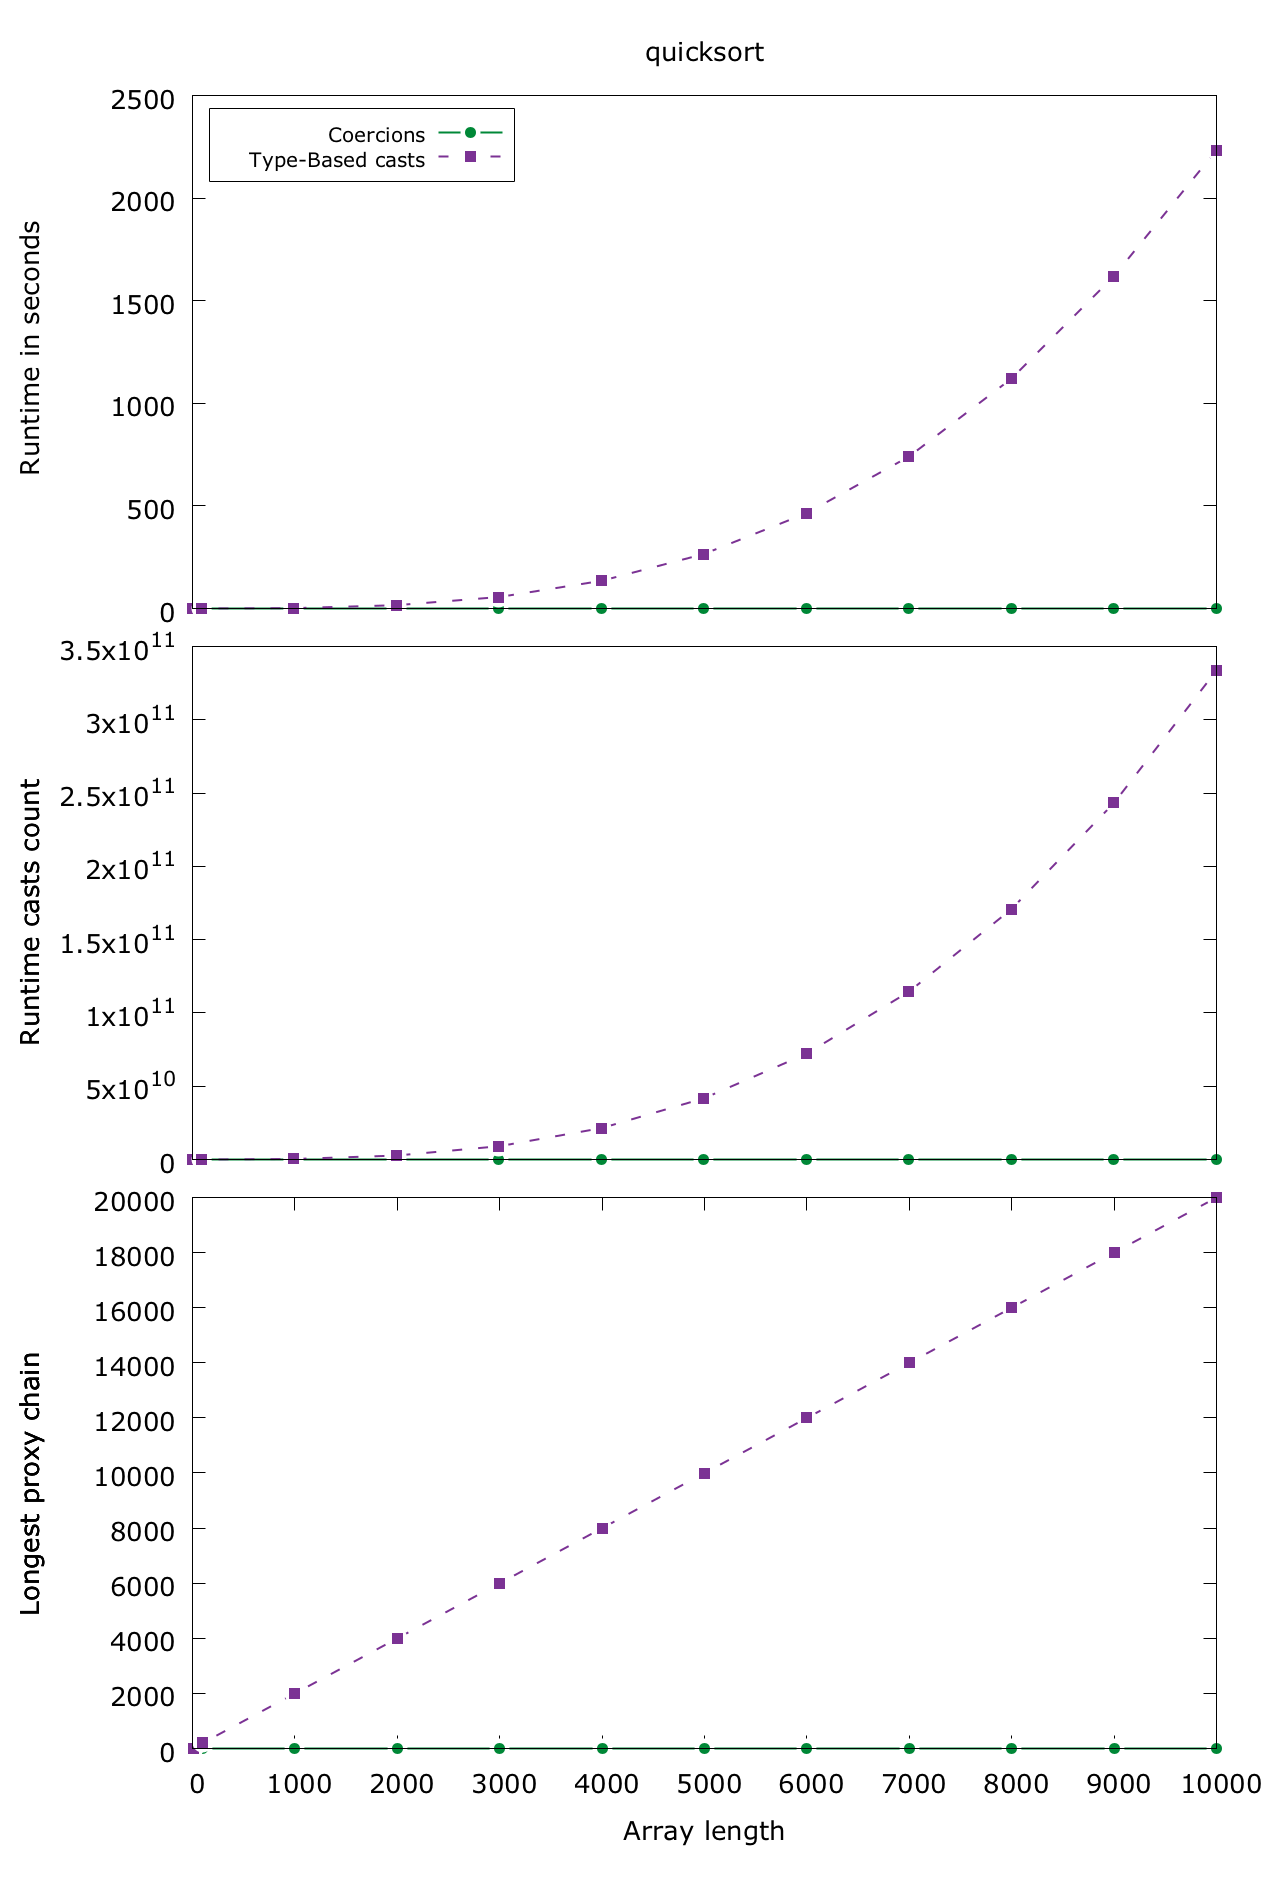
\includegraphics[scale=0.15]{plots/vary-inputs/quicksort.png} \\
\end{center}

}

\frame{
    \[  
    \begin{array}{llcl}
      \text{Coercions}
      & \seCa,\seCb & ::= &
                          \idC \mid \InjectCoercion{T} \mid \ProjectCoercion{T}
                            \mid \FunctionCoercion{\seCa}{\seCb}
                            \mid \FailCoercion{T}{T'}
    \end{array}
  \]

  \begin{itemize}
  \item \customcite{Henglein:1992ys}
  \item \customcite{Herman:2006uq}
  \item \customcite{Siek:2015ab}
  \item they are composable!
  \end{itemize}
  }

\frame{
\frametitle{Research Questions}

\begin{itemize}
\item What is the speed of coercions wrt. regular casts? 
\item What is the overhead for gradual typing on:\\
  (1) statically typed code,\\
  (2) dynamically typed code, and \\
  (3) partially typed code?
\end{itemize}
The theory says $O(1)$, but what is the constant factor?
  
}

\section{Grift Compiler}
\begin{frame}{Outline}
\tableofcontents[currentsection]
\end{frame}
%===============================================================================
\frame{
  \frametitle{The Grift Compiler}

  \begin{itemize}
  \item An ahead-of-time compiler. 23k LOC written in Racket.
  \item The source language GTLC+ includes first-class functions,
    mutable arrays, recursive types, tuples, integers, and floats.
  \item Compiles GTLC+ to C. 
  \item Implements coercions and compose (written in C).
  \item Values are 64 bits. Values of type \DynT are tagged.
  \item Specialize casts if source and target are not \DynT.
  \item Some optimization of function closures (e.g. direct calls).
  \item No global optimizations, no type inference or specialization.
  \item Boehm garbage collector.
  \end{itemize}
}

\section{Performance Evaluation}

\begin{frame}{Outline}
\tableofcontents[currentsection]
\end{frame}
%===============================================================================
\frame{
\frametitle{Situating Grift among Typed Languages}
\begin{center}
  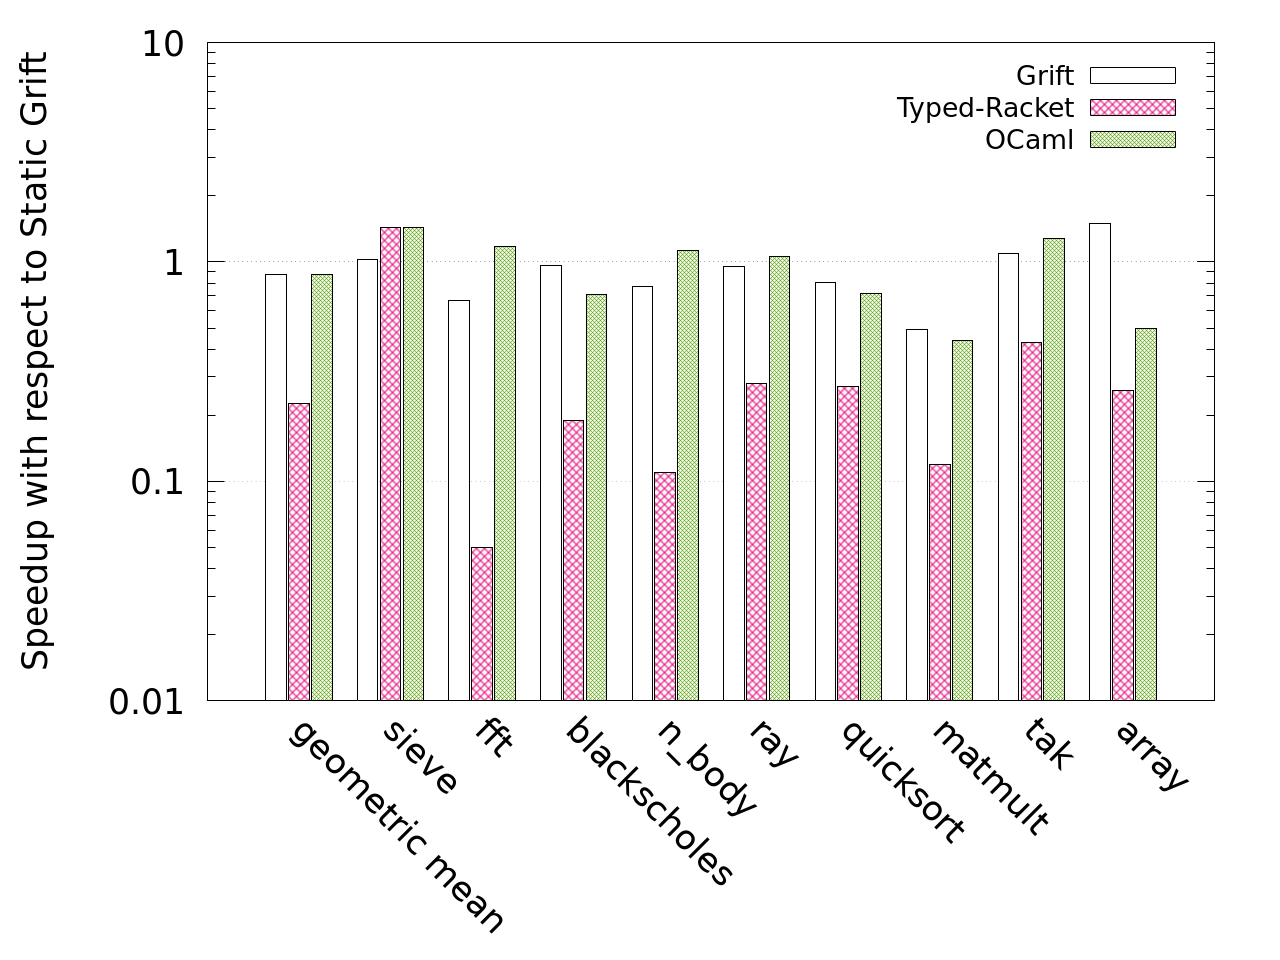
\includegraphics[scale=.23,trim={0 0 0 0},clip]{plots/extremes/Specialized_Lazy_Proxied_Coercions_static.png}
\end{center}
}
%===============================================================================
\frame{
\frametitle{Situating Grift among Untyped Languages}
\begin{center}
  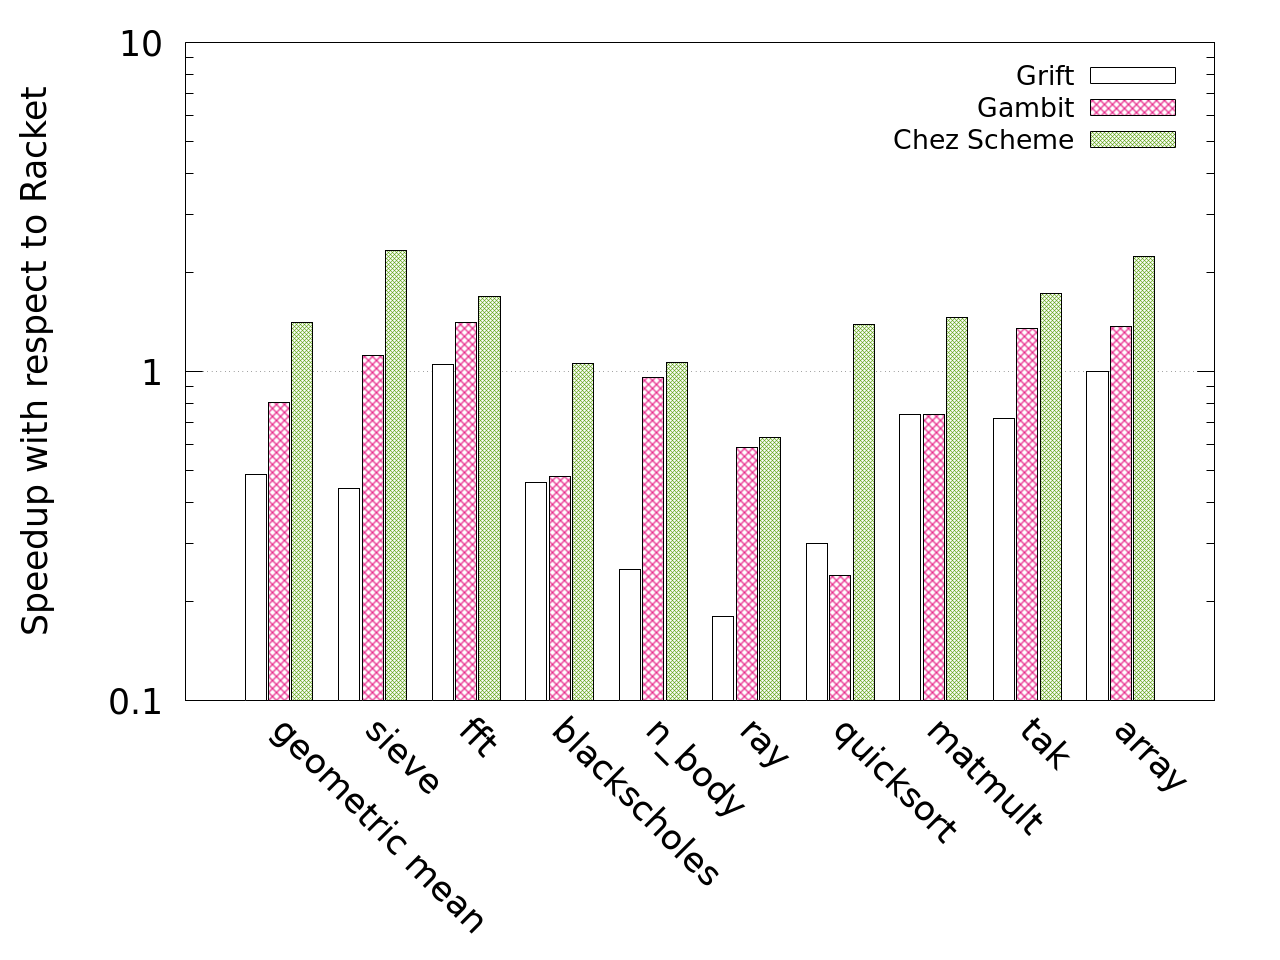
\includegraphics[scale=.23,trim={0 0 0 0},clip]{plots/extremes/Specialized_Lazy_Proxied_Coercions_dynamic.png}
\end{center}
}
%===============================================================================
\frame{
\frametitle{Partially-typed Sieve w/ \& w/o coercions}
\begin{center}
  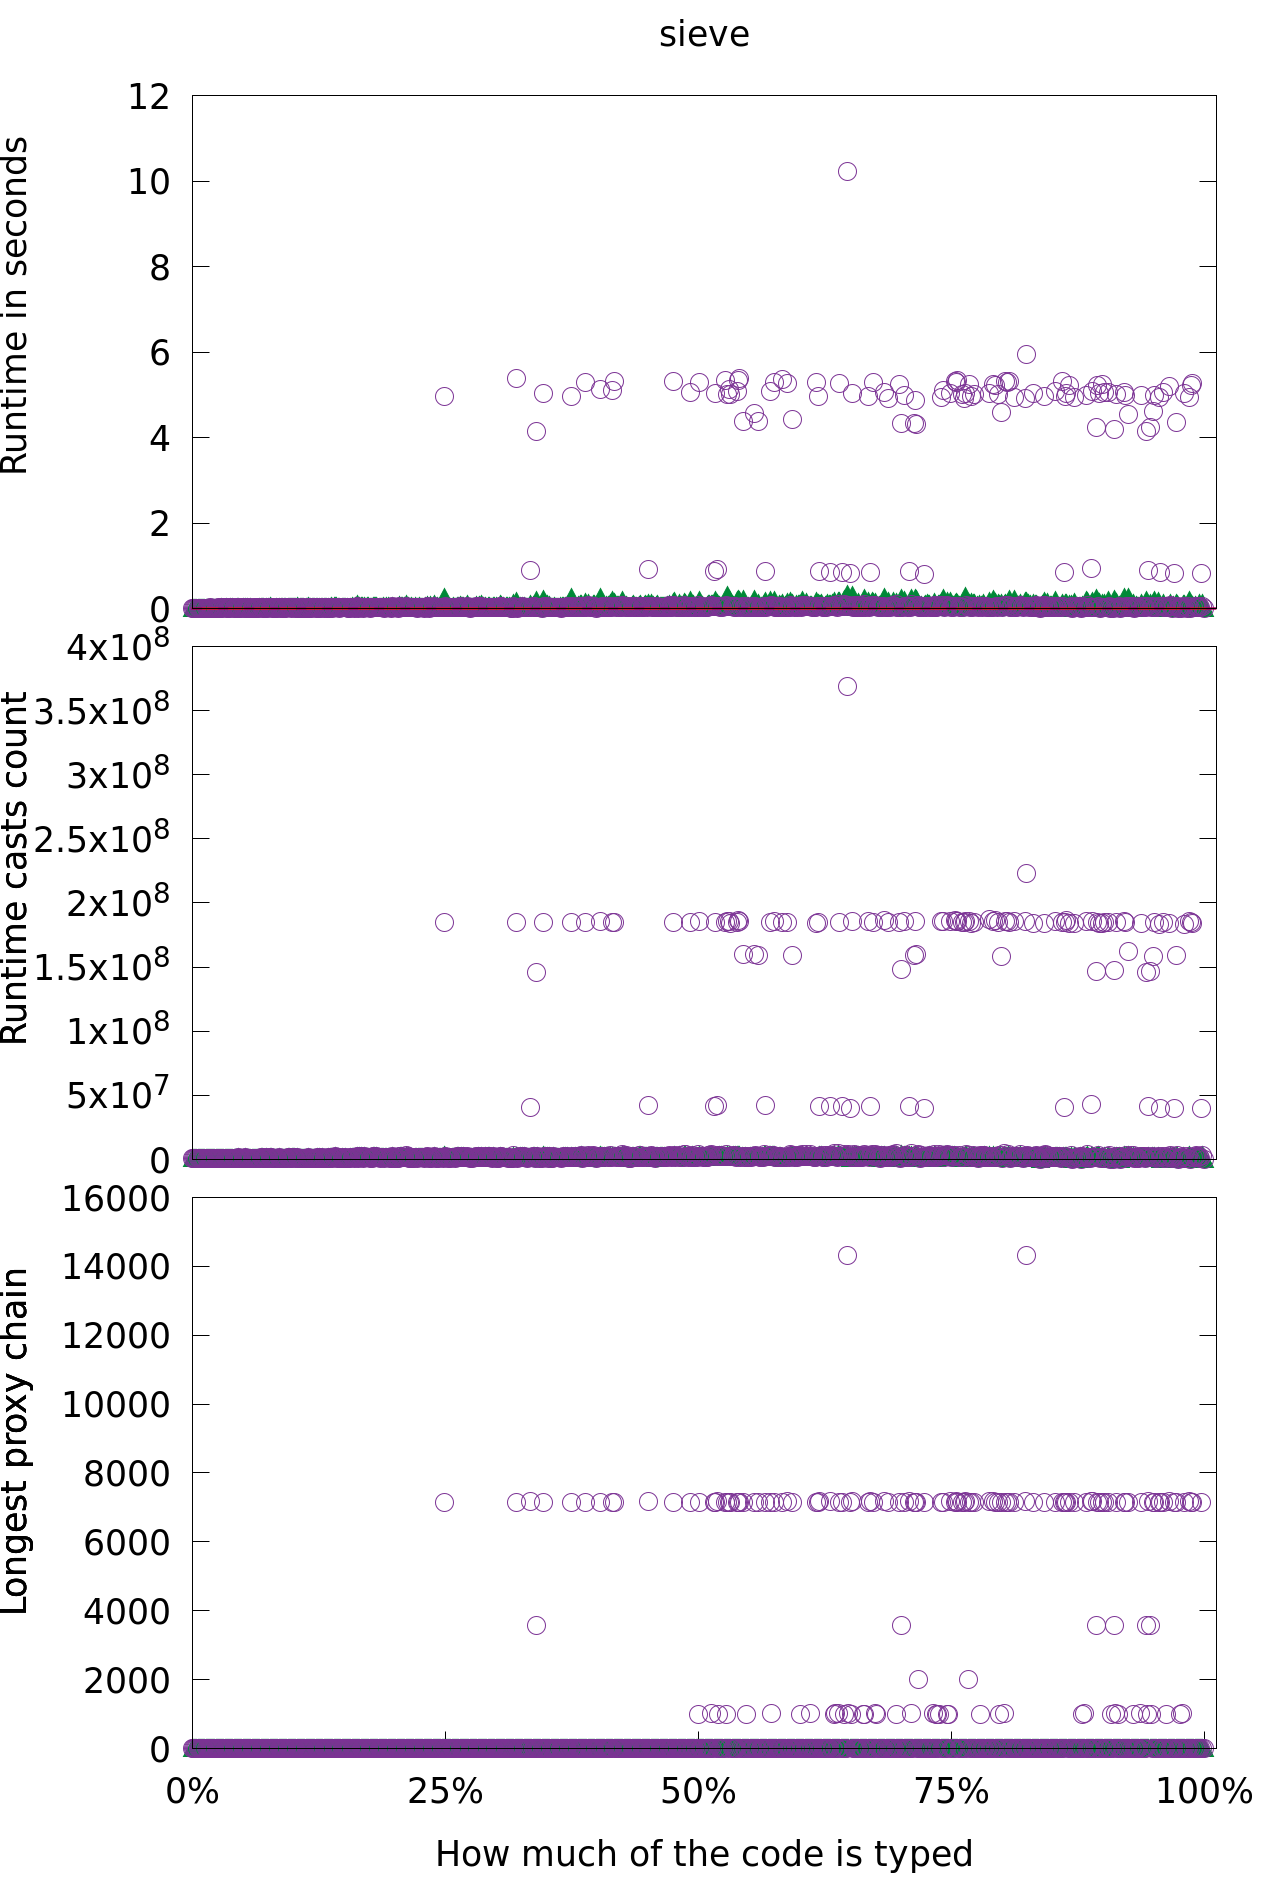
\includegraphics[width=7cm, height=7.75cm]{plots/fine/Proxied_Specialized/all/sieve.png}
\end{center}
}
%===============================================================================
\frame{
\frametitle{Partially-typed N-Body w/ \& w/o coercions}
\begin{center}
  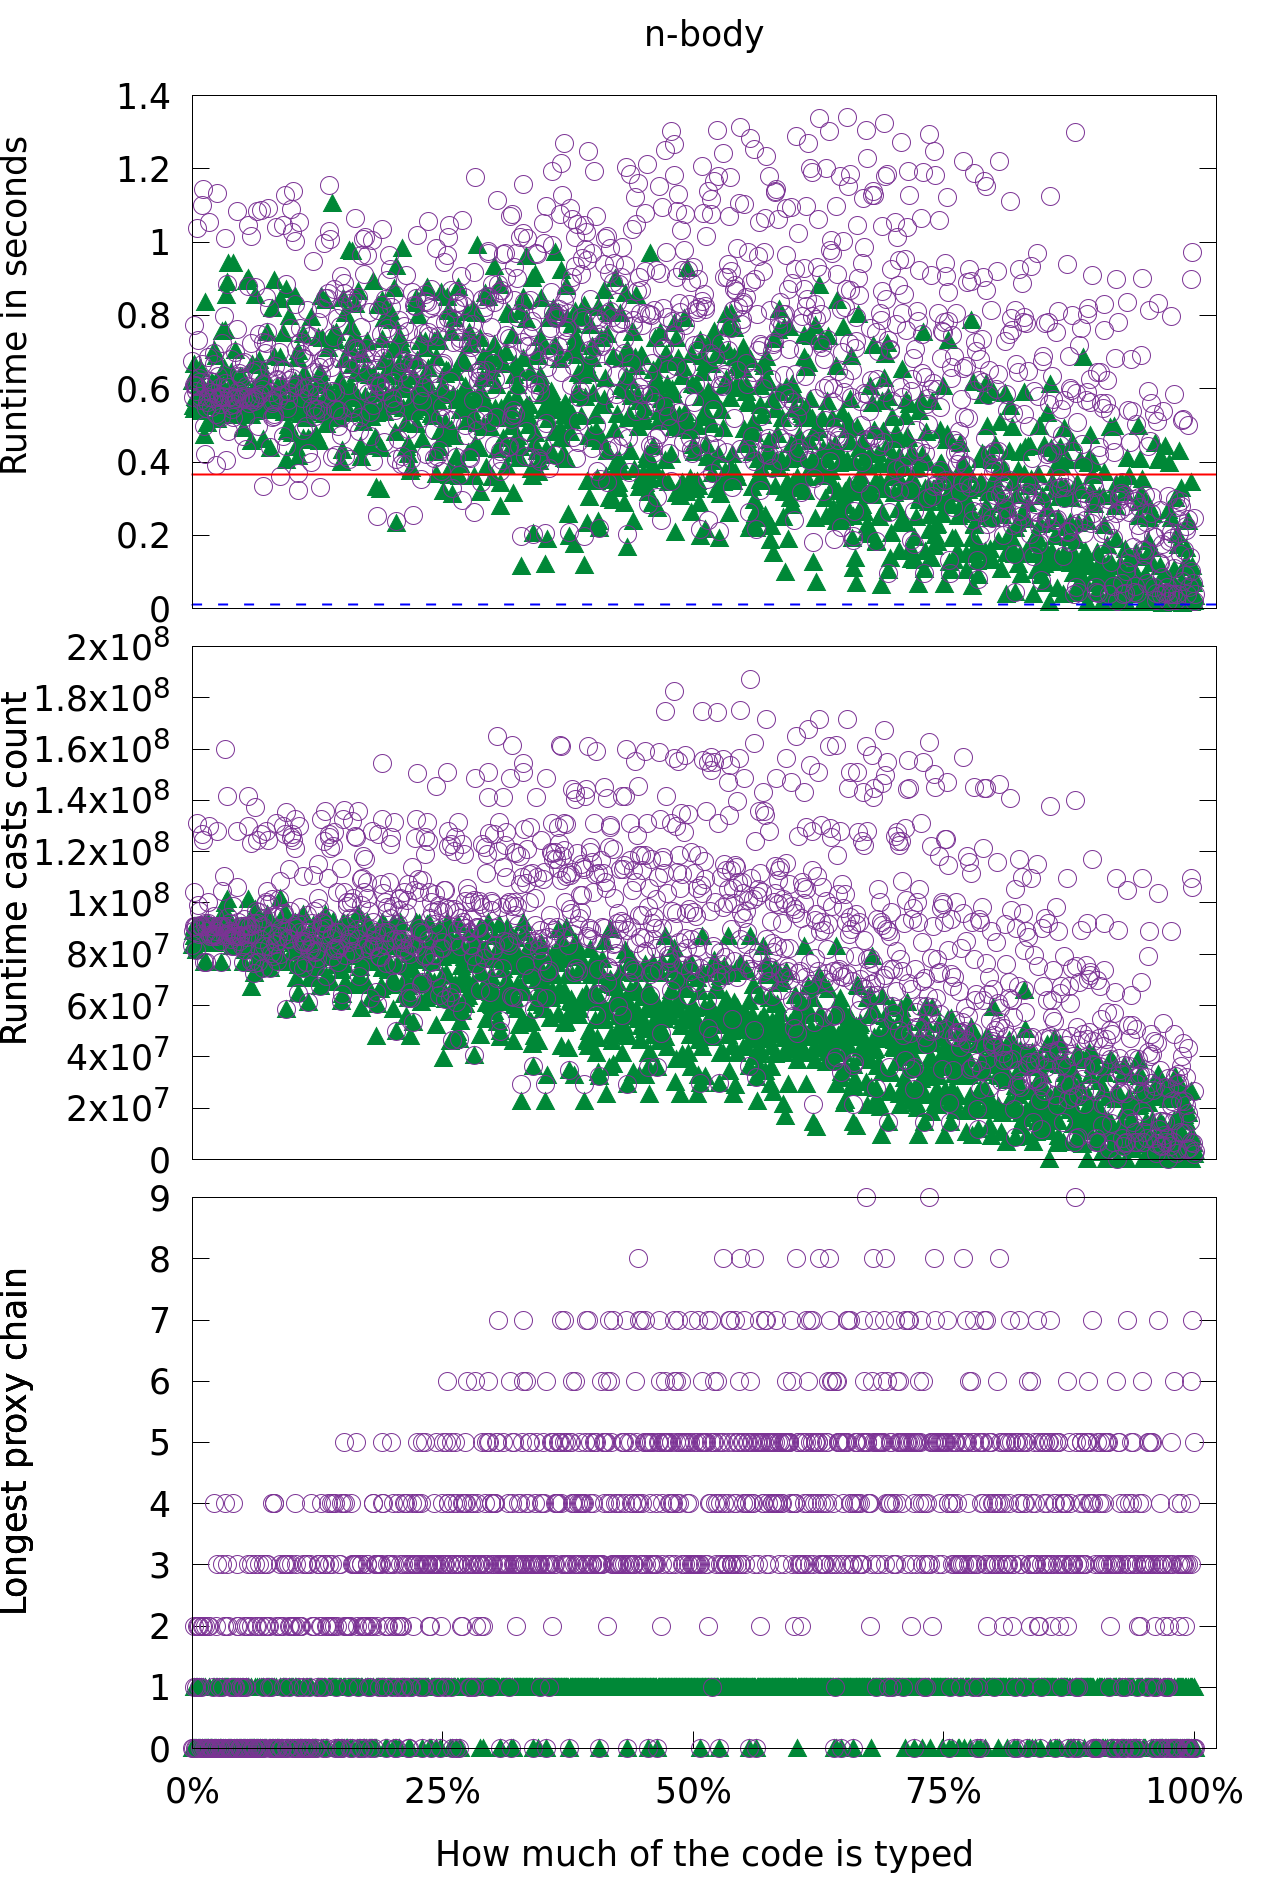
\includegraphics[width=7cm, height=7.75cm]{plots/fine/Proxied_Specialized/all/n_body.png}
\end{center}
}
%===============================================================================
\frame{
\frametitle{Partially-typed Blackscholes w/\&w/o coercions}
\begin{center}
      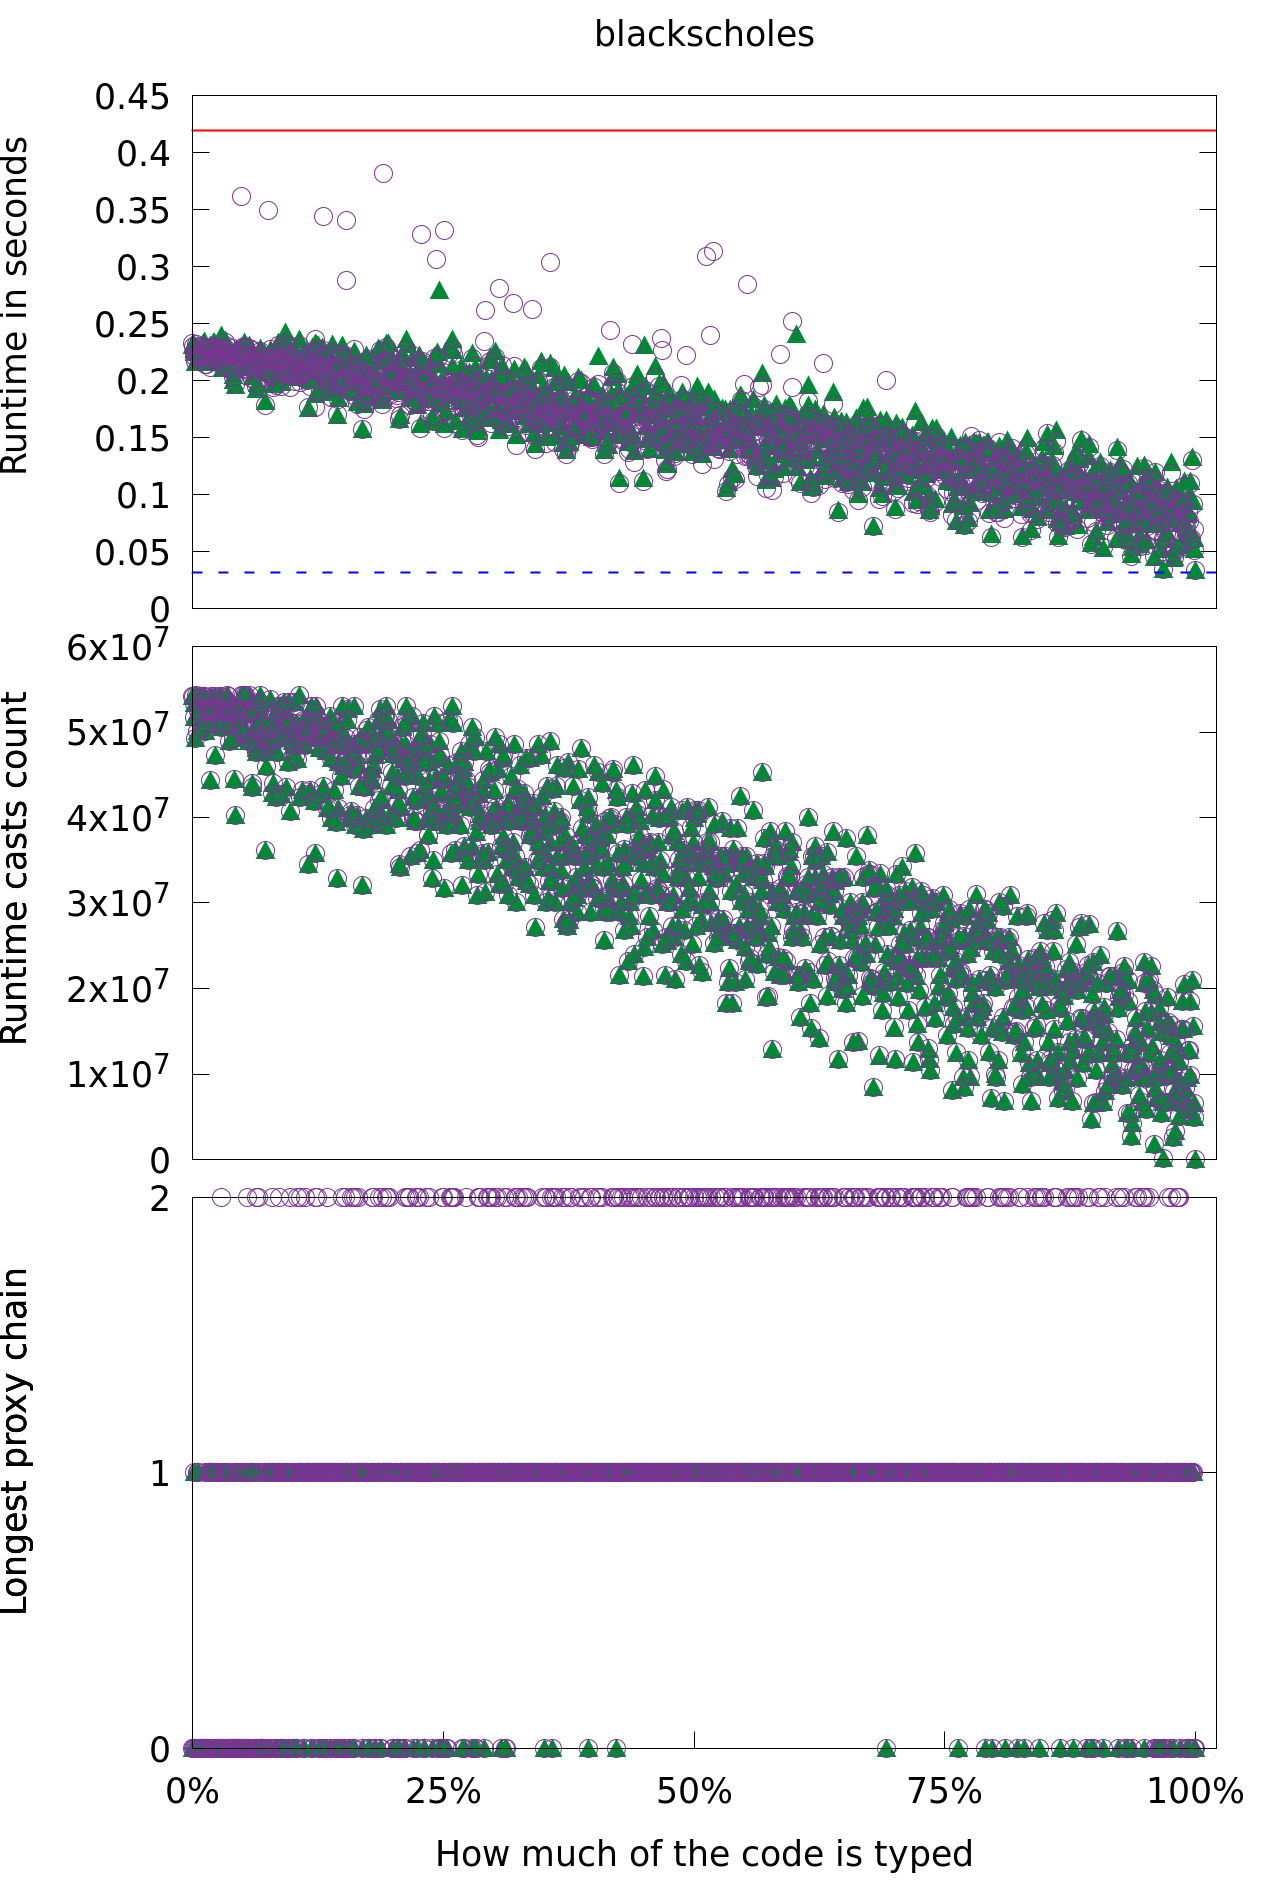
\includegraphics[width=7cm, height=7.75cm]{plots/fine/Proxied_Specialized/all/blackscholes.png}
\end{center}
}

\frame[containsverbatim]{
\frametitle{Comparison to Typed Racket}
\vspace{10pt}
  \begin{tabular}{lr}
      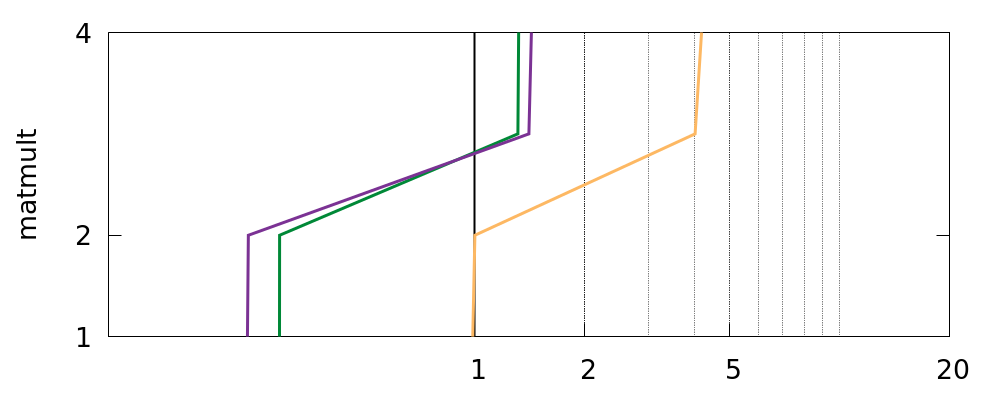
\includegraphics[scale = 0.15]
      {plots/coarse/Proxied_Specialized/cum_perf/matmult.png}
     &
      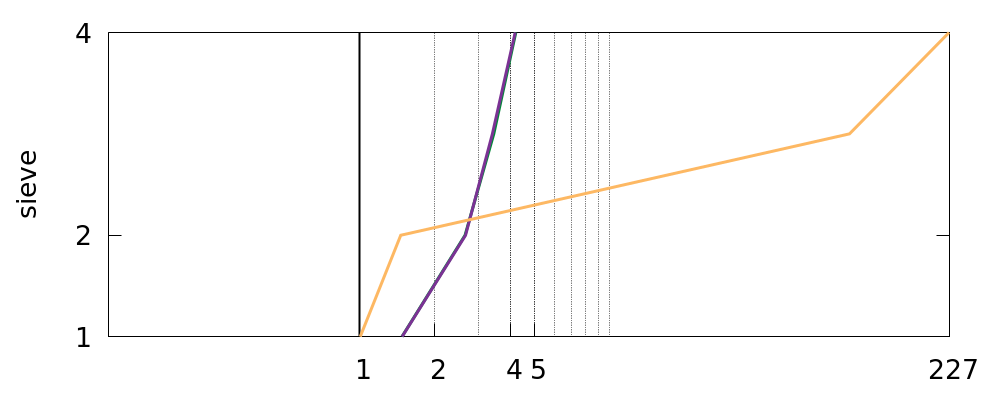
\includegraphics[scale = 0.15]
      {plots/coarse/Proxied_Specialized/cum_perf/sieve.png}
     \\[-1ex]
      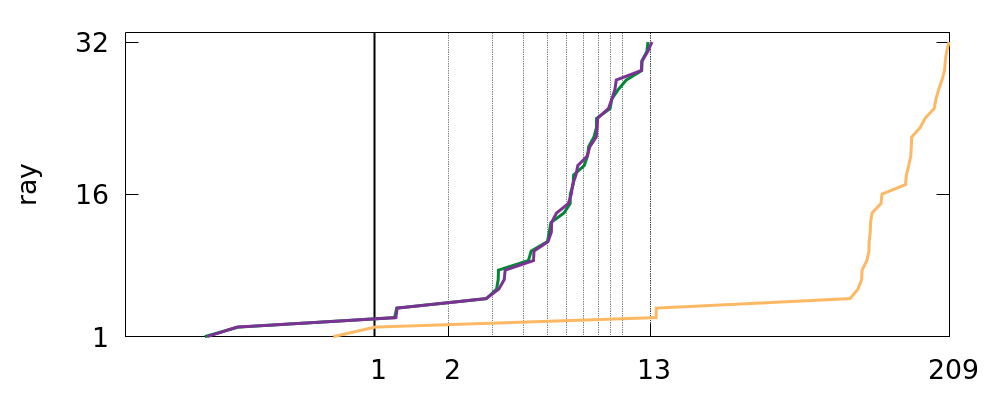
\includegraphics[scale = 0.15]
      {plots/coarse/Proxied_Specialized/cum_perf/ray.png}
     &
      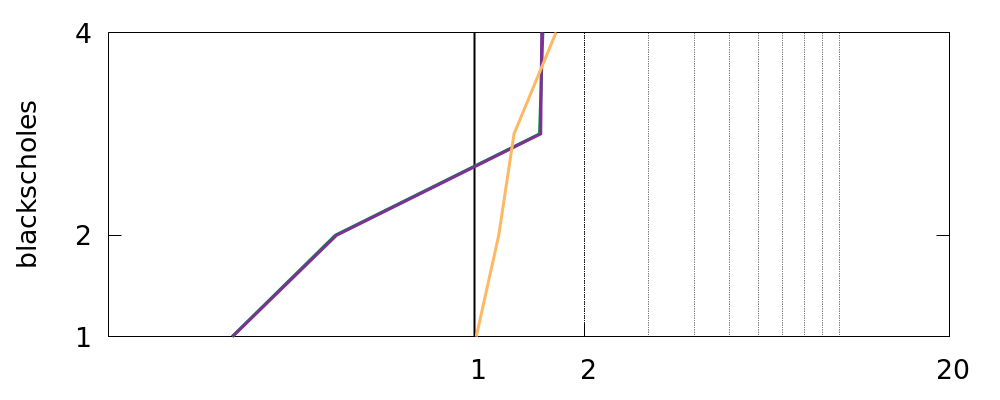
\includegraphics[scale = 0.15]
      {plots/coarse/Proxied_Specialized/cum_perf/blackscholes.png}
     \\[-1ex]
      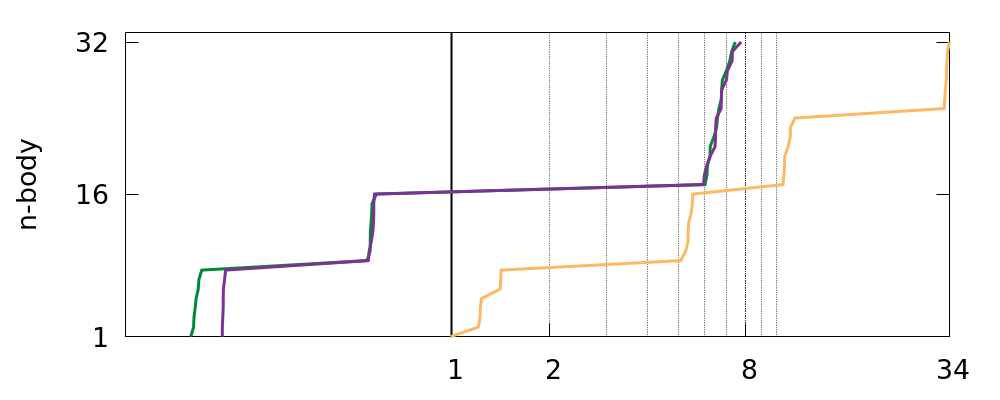
\includegraphics[scale = 0.15]
      {plots/coarse/Proxied_Specialized/cum_perf/n_body.png}
     &
      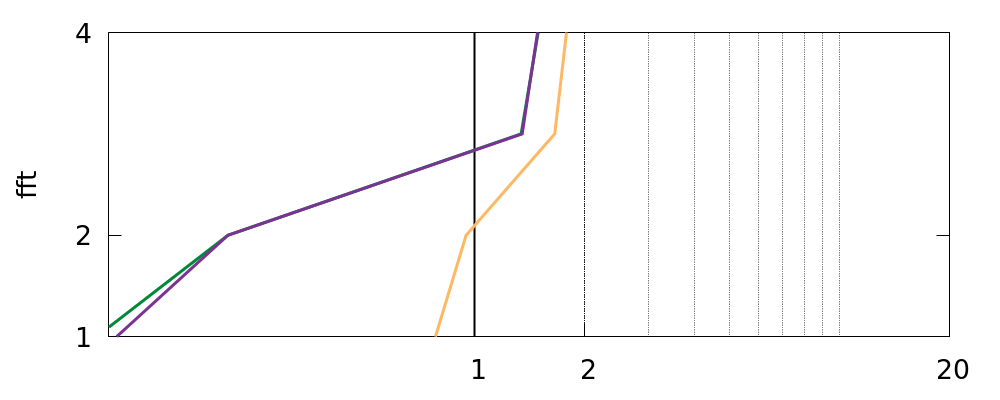
\includegraphics[scale = 0.15]
      {plots/coarse/Proxied_Specialized/cum_perf/fft.png}
  \end{tabular}
  \vspace{-10pt}
  \begin{center}
    
\includegraphics[scale = 0.25]{plots/coarse/Proxied_Specialized/cum_perf/legend.png}
  \end{center}
  \vspace{-10pt}
  {\small X-axis: slowdown wrt. Racket, Y-axis: number of configurations}

}

\frame{
\frametitle{Conclusion}

\begin{itemize}
\item What is the speed with coercions wrt. regular casts? \\
  Much better on programs with proxy-chains.\\
  Similar  on programs without proxy-chains.
  
\item What is the overhead for Grift on:\\
  (1) statically typed code: less than $20\%$ (matmult)\\
  (2) dynamically typed code: $7\times$ (ray), often $<2\times$ \\
  (3) partially typed code: $20\times$ (ray), often $<2\times$

\item Next steps:\\
  -- Improve representation of coercions.\\
  -- Reduce overhead in static code via monotonic pointers.\\
  -- Optimizations such as type inference and inlining.
\end{itemize}

\begin{center}
  \url{https://github.com/Gradual-Typing/Grift}
\end{center}

}
  
\end{document}

%%% Local Variables:
%%% mode: latex
%%% TeX-master: t
%%% End:
